 \documentclass[a4paper,10pt]{article}

\usepackage{amsmath}
\usepackage{amstext}
\usepackage{amssymb}
\usepackage{amsfonts}
\usepackage{amsthm}
\usepackage{etoolbox}
%mathspec/fontspec
\usepackage{mathspec}
\usepackage{xunicode}
\usepackage{xltxtra}

\usepackage[bookmarks,bookmarksnumbered]{hyperref}

\makeatletter       % changes [1] to 1. in bibliography
\renewcommand{\@biblabel}[1]{#1.}
\makeatother

\usepackage{appendix}
\usepackage{graphicx}
\usepackage{natbib}


% FONT
\setmainfont[Mapping=tex-text,Numbers={Lining}]{Linux Libertine O}
\setmathfont(Latin)[Numbers={Lowercase}]{Linux Libertine O}
\setmathfont(Digits)[Scale=MatchLowercase]{Linux Libertine O}

\usepackage{unicode-math}
\setmainfont[Mapping=tex-text,Numbers={Lining}]{Linux Libertine O} 
\setmathfont{XITS Math}

\setmathfont[range={\mathup}]{Linux Libertine O} 
\setmathfont[range={\mathit}]{Linux Libertine O Italic} 
\setmathfont[range={\rm}]{Linux Libertine O} 
\setmathfont[range={\mathrm}]{Linux Libertine O} 



% \renewcommand{\rmdefault}{fxl}
\renewcommand{\sfdefault}{txss}


%%%%%%%%% from here yuasa setting %%%%%%%%%%%%%%%%%%%%%
% a4paper paperheight = 845.04684pt
%\setlength{\topmargin}{-.5in}
%% textheight = paperheight - 2in - \topmargin - \headheight - \headsep
%%              - \footskip = approx. 641pt
%\setlength{\textheight}{1.05\paperheight}
%\addtolength{\textheight}{-2.2in}
%%\addtolength{\textheight}{-\topmargin}
%%\addtolength{\textheight}{-\headheight}
%%\addtolength{\textheight}{-\headsep}
%%\addtolength{\textheight}{-\footskip}

%% a4paper paperwidth = 597.50787pt
%%\setlength{\marginparsep}{0pt}
%%\setlength{\marginparwidth}{0pt}
%% textwidth = paperwidth - 2in - \oddsidemargin = approx. 432pt
%\setlength{\textwidth}{\paperwidth}
%\addtolength{\textwidth}{-1.8in}
%%\addtolength{\textwidth}{-\oddsidemargin}

%% add 20pt to sidemargin
%%   oddside: 1in+20pt+20pt | \textwidth | 1in-20pt
%%   evenside: 1in-20pt | \textwidth | 1in+20pt+20pt
%\setlength{\oddsidemargin}{0pt}
%\setlength{\evensidemargin}{0pt}

%%%%%%%%% to here yuasa setting %%%%%%%%%%%%%%%%

%%%%%%%%% from here margin setting %%%%%%%%%%%%%%%%
%for dron
%\setlength{\topmargin}{0pt}
%\setlength{\marginparsep}{0pt}
%\setlength{\marginparwidth}{0pt}
%\setlength{\oddsidemargin}{20pt}
%\setlength{\evensidemargin}{0pt}
%
%\setlength{\textwidth}{\paperwidth}
%\addtolength{\textwidth}{-2in}
%\addtolength{\textwidth}{-\oddsidemargin}
%
%\addtolength{\oddsidemargin}{0pt}
%\addtolength{\evensidemargin}{-23pt}
%\setlength{\topmargin}{-12mm}
%\setlength{\textheight}{25.3cm}
%\setlength{\textwidth}{16.3cm}
%%%%%%%%% till here margin setting %%%%%%%%%%%%%%%%

%%% Linestrech
%for user guide
\renewcommand{\baselinestretch} {1.1}
%for dron
%\renewcommand{\baselinestretch} {1.1}

\setlength\bibsep{2pt}
\renewcommand{\bibnumfmt}[1]{(#1)}


%%% Table of Contents
\usepackage{tocloft}
\setlength\cftparskip{-0.7pt}
\setlength\cftbeforesecskip{1.5pt}
\setlength\cftaftertoctitleskip{2pt}

\addtolength{\oddsidemargin}{-.875in}
	\addtolength{\evensidemargin}{-.875in}
	\addtolength{\textwidth}{1.75in}

	\addtolength{\topmargin}{-.875in}
	\addtolength{\textheight}{1.75in}

%% for quotes
%\fontspec[Mapping=tex-text]{Linux Libertine O}
%\fontspec[Ligatures=TeX]{Linux Libertine O}

%%%%%%%%% color %%%%%%%%%
\usepackage{color}
\newcommand{\red}{\textcolor{red}}
\newcommand{\green}{\textcolor{green}}
\newcommand{\blue}{\textcolor[rgb]{0,0,0.8}}
\newcommand{\midnightblue}{\textcolor[rgb]{0.0976,0.0976,0.4375}}
\newcommand{\apricot}{\textcolor[rgb]{1,0,0.5}}
\newcommand{\strawberry}{\textcolor[rgb]{1,0,0.5}}
\newcommand{\orange}{\textcolor[rgb]{0.949, 0.593, 0}}
\newcommand{\gray}{\textcolor[rgb]{0.4,0.4,0.4}}
%%%%%%%%%%%%%%%%%%%%%%%%%%%


%%%%%%%%% for source code listing %%%%%%%%%
\usepackage{listings}


\lstset{%
 language={XML},
 backgroundcolor={\color[gray]{.97}},%
 basicstyle={\small\ttfamily},%
% identifierstyle={\small\ttfamily},%
 commentstyle={\gray},%
% keywordstyle={\small\bfseries\ttfamily},%
% ndkeywordstyle={\small},%
% stringstyle={\apricot},
 frame={tb},
 breaklines=true,
% columns=[l]{fullflexible},%
 numbers=left,%
% xrightmargin=5pt,%
% xleftmargin=5pt,%
% numberstyle={\scriptsize},%
% stepnumber=1,
 numbersep=5pt,%
 lineskip=-0.5pt,%
 showstringspaces=false,
 numbers=none
}
%%%%%%%%%%%%%%%%%%%%%%%%%%%

\title{\Huge{
SpaceWire RMAP GUI}\\
\Large{User Guide}}

\author{
{\Large
Takayuki Yuasa
}\\
{\small Japan Aerospace Exploration Agency, Institute of Space and Astronautical Science}\\
}

\date{December, 2011}

\newcommand{\red}{\textcolor{red}}
\newcommand{\green}{\textcolor{green}}
\newcommand{\blue}{\textcolor{blue}}
\newcommand{\apricot}{\textcolor[rgb]{1,0,0.5}}

\usepackage{listings}
\usepackage{color}

\lstset{%
 language={XML},
 backgroundcolor={\color[gray]{.97}},%
 basicstyle={\small\ttfamily},%
 identifierstyle={\small\ttfamily},%
 commentstyle={\small\ttfamily\itshape},%
 keywordstyle={\small\bfseries\ttfamily},%
 ndkeywordstyle={\small},%
 stringstyle={\small\ttfamily\apricot},
 frame={tb},
 breaklines=true,
% columns=[l]{fullflexible},%
 numbers=left,%
 xrightmargin=5pt,%
 xleftmargin=5pt,%
% numberstyle={\scriptsize},%
% stepnumber=1,
 numbersep=5pt,%
 lineskip=-0.5pt%
}

\begin{document}
\maketitle
\tableofcontents

\setcounter{page}{2}

%%%%%%%%%%%%%%%%%%%%%%%%%%%%%%%%%%%%%%
%%%%%%%%%%%%%%%%%%%%%%%%%%%%%%%%%%%%%%
\section{Overview of SpaceWire RMAP GUI}
SpaceWire RMAP GUI is an easy-to-use graphical user interface front end for SpaceWire-to-GigabitEther. The software runs on Mac OS X, and is capable of sending and receiving raw SpaceWire packets, and performing RMAP\footnote{Remote Memory Access Protocol.} read/write transactions using a SpaceWire interface connected to your Mac. SpaceWire-to-GigabitEther is a default SpaceWire interface supported by SpaceWire RMAP GUI. 
In addition to these, RMAP packet construction/interpretation is provided. The software is developed as an open-source project, and contributions and/or feedbacks from users or developers are highly appreciated.

Several types of information used in SpaceWire RMAP GUI, such as RMAP target node information, memory object on an RMAP target node, can be defined using XML-like file. By loading definition files, users do not need to input logical address, target SpaceWire address, memory address, length, or other properties every RMAP access.

As shown in Figure \ref{figure:tab_rmap}, the main window consists of three tabs which displays SpaceWire, RMAP, and RMAP packet utility functionalities.
\begin{figure}[htb]
%\rotatebox{90}{\begin{minipage}{\textheight}
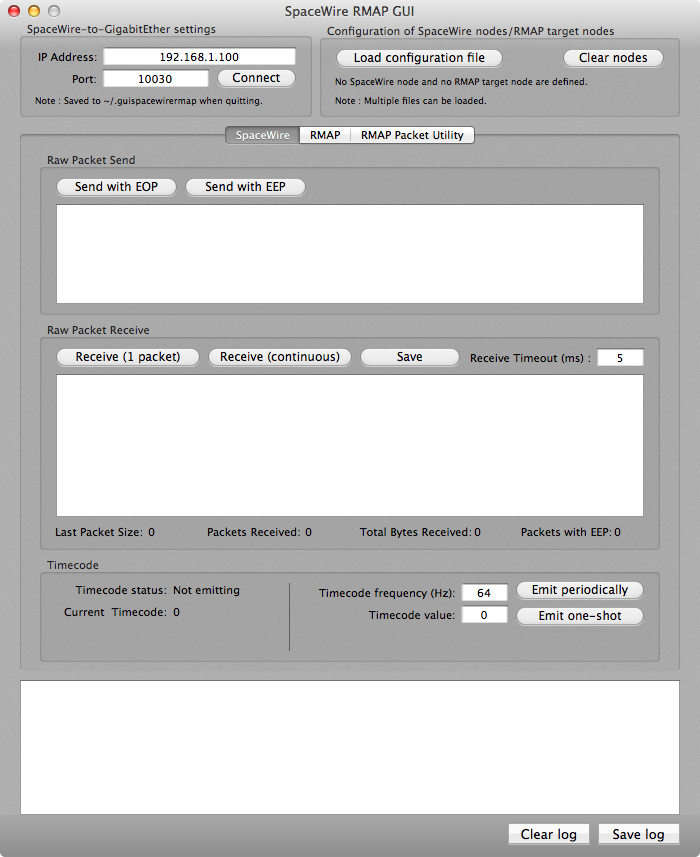
\includegraphics[width=8cm]{figures/SpaceWireRMAPGUI/Screenshot_Tab_SpaceWire.png}
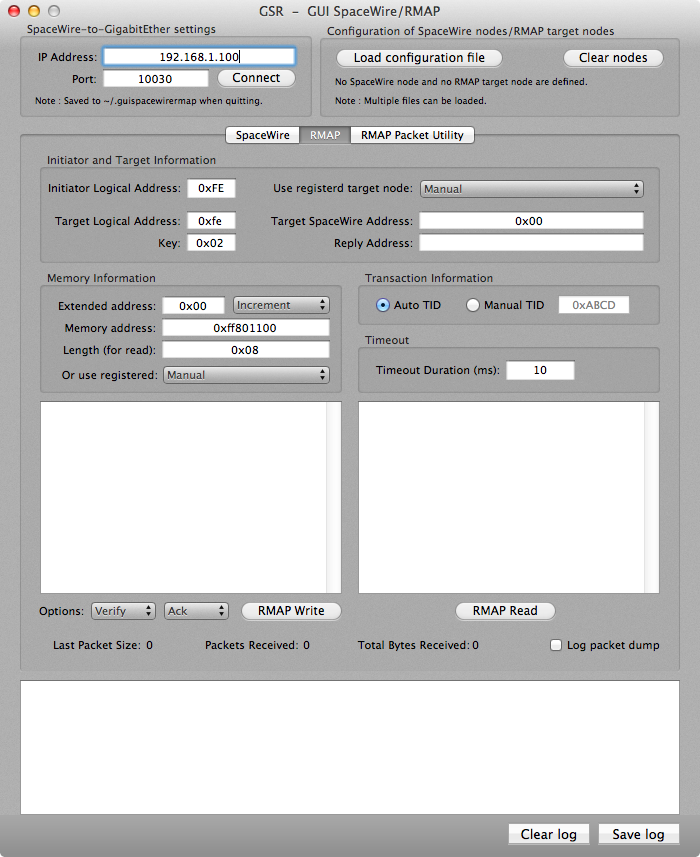
\includegraphics[width=8cm]{figures/SpaceWireRMAPGUI/Screenshot_Tab_RMAP.png}
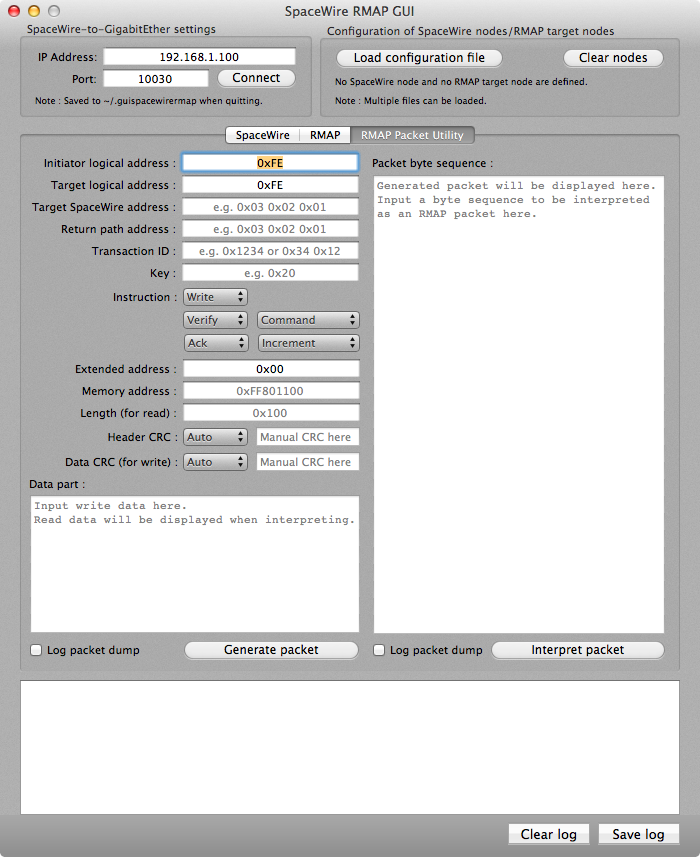
\includegraphics[width=8cm]{figures/SpaceWireRMAPGUI/Screenshot_Tab_RMAPPacketUtility.png}
\caption{Screenshots of each function of SpaceWire RMAP GUI.}
\label{figure:tab_rmap}
%\end{minipage}}
\end{figure}

SpaceWire RMAP GUI uses libraries listed below:
\begin{itemize}
  \setlength{\parskip}{0cm}
  \setlength{\itemsep}{0cm}
\item SpaceWire/RMAP Library\footnote{https://github.com/yuasatakayuki/SpaceWireRMAPLibrary}
\item CxxUtilities\footnote{https://github.com/sakuraisoki/XMLUtilities/}
\item XMLUtility by Soki Sakurai from The University of Tokyo\footnote{https://github.com/sakuraisoki/XMLUtilities/}
\item xerces-c++ by the Apache project\footnote{http://xerces.apache.org/xerces-c/}
\end{itemize}
These libraries are statically linked to the software, and therefore, users are not required to install individual libraries separately.

Note that the software is distributed for free assuming that this is useful for some users without any warranty or official support, and developers are not responsible for any damages caused by this software.

\clearpage

%%%%%%%%%%%%%%%%%%%%%%%%%%%%%%%%%%%%%%
%%%%%%%%%%%%%%%%%%%%%%%%%%%%%%%%%%%%%%
\section{About this user guide}
The user guide is provided {\it as is} expecting that this is somewhat useful for users to use the software. This is a voluntary mission, and therefore, kind help is always welcome. It is greatly appreciated to make contributions by feed-backing comments, revising documents, and so on.

\subsection{Latest information and feedback}
Latest information on SpaceWire RMAP GUI and SpaceWire-to-GigabitEther can be found at the open-source SpaceWire project website \footnote{The open-source SpaceWire project: https://galaxy.astro.isas.jaxa.jp/~yuasa/SpaceWire\label{url:supportpage}}.

\subsection{References}
Documents listed below can be a nice reference when better understanding SpaceWire RMAP GUI. Some of the documents can be obtained from the open-source SpaceWire project website$^\mathrm{\ref{url:supportpage}}$.
\begin{itemize}
  \setlength{\parskip}{0cm}
  \setlength{\itemsep}{0cm}
\item SpaceWire/RMAP Library User Guide
\item SpaceWire-to-GigabitEther User Guide
\item ECSS-E-ST-50-12C - "SpaceWire - Links, nodes, routers and networks" by ECSS
\item ECSS-E-ST-50-52C "SpaceWire - Remote memory access protocol" by ECSS
\end{itemize}

\subsection{Revisions}
\begin{itemize}
  \setlength{\parskip}{0cm}
  \setlength{\itemsep}{0cm}
\item 2012-01-01 Takayuki Yuasa. First release.
\end{itemize}



%%%%%%%%%%%%%%%%%%%%%%%%%%%%%%%%%%%%%%
%%%%%%%%%%%%%%%%%%%%%%%%%%%%%%%%%%%%%%
\section{Overall structure of SpaceWire RMAP GUI}
SpaceWire RMAP GUI displays single main window when start up.
The window contains three tabs (or panels), and each tab collects text fields and buttons which are necessary for SpaceWire, RMAP, and RMAP Packet Utility functions.

\subsection{The main window}
The main window is divided into four sections; the SpaceWire-to-GigabitEther setting section (top left; see Section \ref{section:setting_section}), the configuration file section (top right; see Section \ref{section:configuration_section}), the main tab (middle), and the log message section (bottom). When the main window is closed, SpaceWire RMAP GUI quits. If SpaceWire-to-GigabitEther is connected via TCP/IP when quitting, SpaceWire RMAP GUI tries to close the connection. Settings (values contained in each input fields) are saved to the preference file, and loaded again at the start up.

\subsection{SpaceWire tab}
The SpaceWire tab allows users to handle raw SpaceWire packets.
Periodic or ordered timecode emission is managed from this tab as well.

\subsection{RMAP tab}

\subsection{RMAP Packet Utility tab}

\subsection{Typical procedure}
When analyzing/creating RMAP packets in the RMAP Packet Utility tab, no connection to SpaceWire-to-GigabitEther is necessary.
When sending/receiving SpaceWire packets or initiating RMAP read/write, follow the procedure below:
\begin{enumerate}
  \setlength{\parskip}{0cm}
  \setlength{\itemsep}{0cm}
\item Set the IP address and the TCP port number.
\item Click the "Connect" button.
\item Load XML configuration files (to register RMAP Target Node information) if needed.
\item Send/receive SpaceWire packets (from the SpaceWire tab), \\
or initiate RMAP read/write (from the RMAP tab).\\
\end{enumerate}




%%%%%%%%%%%%%%%%%%%%%%%%%%%%%%%%%%%%%%
%%%%%%%%%%%%%%%%%%%%%%%%%%%%%%%%%%%%%%
\section{Settings}
\subsection{TCP/IP connection to SpaceWire-to-GigabitEther}\label{section:setting_section}
SpaceWire RMAP GUI should be used with SpaceWire-to-GigabitEther which provides a physical connection to SpaceWire network via TCP/IP over GigabitEthernet. The device can be purchased from Shimafuji Electric as a paid product, or an open-source (free) version on commercial FPGA board (ZestET1 by OrangeTree) is available from the open-source SpaceWire project.

Users can set an IP address (or URL) and utilized port number of SpaceWire-to-GigabitEther in the section on top-left of the main window as shown in Figure \ref{figure:section_SpaceWire-to-GigabitEther}. When the "Connect" button is clicked, the software tries to connect to the specified SpaceWire-to-GigabitEther, and then SpaceWire packet sending/receiving and RMAP initiator functions become available if a connection is successfully established. If timeout occurs, an error dialog will be displayed.

\begin{figure}[htb]
\begin{center}
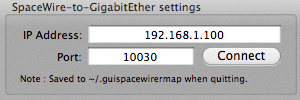
\includegraphics[height=2.5cm]{figures/SpaceWireRMAPGUI/Section_SpaceWire-to-GigabitEther_settings.png}
\caption{Input files for the IP address and the TCP port number of SpaceWire-to-GigabitEther.}
\label{figure:section_SpaceWire-to-GigabitEther}
\end{center}
\end{figure}

Note: Port number selects SpaceWire port of the internal SpaceWire router (when available on your SpaceWire-to-GigabitEther device). The default value 10030 may correspond to port 6 in Shimafuji's SpaceWire-to-GigabitEther, and port 1 in open-source SpaceWire-to-GigabitEther (which does not implement an internal router, and the port is directly connected to the physical connector on the board).

Note: As written on the window, the IP address and TCP port number will be saved to an invisible configuration file "~/.guispacewirermap". Other settings such as default RMAP header information, will be saved to a preference file which is located in the OS X default folder (~/Library/Preferences/).

\subsection{RMAP Target Node definition using XML-like files}\label{section:configuration_section}
In SpaceWire RMAP GUI, an XML-like text file or files is/are used to load RMAP target node information such as a logical address, target SpaceWire address and reply address, and memory object (or register) information on the RMAP target node such as memory address, access length, access modes. This allows users to deal  with a large network which consists of large number of RMAP target nodes by avoiding manual reconfiguration of many input fields in the RMAP tab in every RMAP access.

The example shown below tells typical syntax used to define an RMAP Target Node and memory objects on it.  See SpaceWire/RMAPLibrary User Guide for details of the format.

\begin{lstlisting}[label=source:xml_configurationfile_example, caption=An example of an XML-like configuration file.]
<root>

<RMAPTargetNode id="SpaceWireToGigabitEther_RouterConfigurationPort">
	<TargetLogicalAddress>0xFE</TargetLogicalAddress>
	<TargetSpaceWireAddress>0x00</TargetSpaceWireAddress>
	<ReplyAddress></ReplyAddress>
	<Key>0x20</Key>

	<RMAPMemoryObject id="Port1ControlStatusRegister">
		<ExtendedAddress>0x00</ExtendedAddress>
		<Address>0x0000</Address>
		<Length>0x04</Length>
		<Key>0x20</Key>
	</RMAPMemoryObject>

	<RMAPMemoryObject id="Port2ControlStatusRegister">
		<ExtendedAddress>0x00</ExtendedAddress>
		<Address>0x0000</Address>
		<Length>0x08</Length>
		<Key>0x20</Key>
	</RMAPMemoryObject>

	<RMAPMemoryObject id="RouterID">
		<ExtendedAddress>0x00</ExtendedAddress>
		<Address>0x404</Address>
		<Length>0x04</Length>
		<Key>0x20</Key>
	</RMAPMemoryObject>
</RMAPTargetNode>

<RMAPTargetNode id="SpaceWireToGigabitEther_RegisterPort">
	<TargetLogicalAddress>0xFE</TargetLogicalAddress>
	<TargetSpaceWireAddress>0x09</TargetSpaceWireAddress>
	<ReplyAddress>0x04</ReplyAddress>
	<Key>0x20</Key>	
</RMAPTargetNode>

</root>
\end{lstlisting}

By loading configuration files from the "Configuration" section in the main window which is shown in Figure \ref{figure:section_ConfigurationFiles}, defined RMAP Target Nodes will be listed in the pull-down menu in "Initiator and Target Information" section of the RMAP tab. When one of defined RMAP Target Node is selected, its information is automatically set to relevant input fields, and correspondingly memory objects will be displayed in the register name pull-down menu in the "Memory Information" section. When selecting an entry from the register name pull-down menu, memory address and length will be automatically set.
\begin{figure}[htb]
\begin{center}
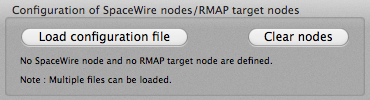
\includegraphics[height=2.5cm]{figures/SpaceWireRMAPGUI/Section_LoadConfigurationFile.png}
\caption{Configuration file section.}
\label{figure:section_ConfigurationFiles}
\end{center}
\end{figure}

The above example results with RMAP Target Nodes named "SpaceWireToGigabitEther\_RouterConfigurationPort" and "SpaceWireToGigabitEther\_RegisterPort", and memory objects on "SpaceWireToGigabitEther\_RouterConfigurationPort" named "Port1ControlStatusRegister", "Port2ControlStatusRegister", and "RouterID" each having 4-byte fields. Figure \ref{figure:section_pull-down_menus} shows a screenshot of the RMAP Target Node pull-down menu and the register pull-down menu in the RMAP tab after loading the configuration file.
\begin{figure}[htb]
\begin{center}
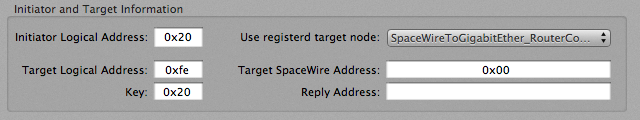
\includegraphics[height=2.5cm]{figures/SpaceWireRMAPGUI/Section_InitiatorAndTargetInformation_with_registered_RMAPTargetNode.png}\\\vspace{2mm}
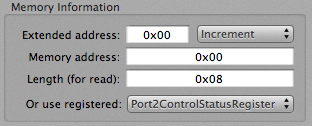
\includegraphics[height=2.5cm]{figures/SpaceWireRMAPGUI/Section_MemoryInformation_with_registered_MemoryObject.png}
\caption{The Initiator and Target Information section (top) and the Memory Information section (bottom) after loading the example XML configuration file, and selecting one of the defined entries in each pull-down menu.}
\label{figure:section_pull-down_menus}
\end{center}
\end{figure}

%%%%%%%%%%%%%%%%%%%%%%%%%%%%%%%%%%%%%%
%%%%%%%%%%%%%%%%%%%%%%%%%%%%%%%%%%%%%%
\section{SpaceWire}
\subsection{Sending packets}
\subsection{Receiving packets}
\subsection{Emitting timecode}
\subsection{Errors and timeout}

%%%%%%%%%%%%%%%%%%%%%%%%%%%%%%%%%%%%%%
%%%%%%%%%%%%%%%%%%%%%%%%%%%%%%%%%%%%%%
\section{RMAP}
\subsection{Performing Write}
\subsection{Performing Read}
\subsection{Errors and timeout}
\subsection{Use defined RMAP Target Nodes and memory objects}


%%%%%%%%%%%%%%%%%%%%%%%%%%%%%%%%%%%%%%
%%%%%%%%%%%%%%%%%%%%%%%%%%%%%%%%%%%%%%
\section{RMAP Packet Utility}
\subsection{Creating RMAP packets}
\subsection{Interpreting RMAP packets}
\subsection{Errors}
\subsubsection{CRC error}




%%%%%%%%%%%%%%%%%%%%%%%%%%%%%%%%%%%%%%
%%%%%%%%%%%%%%%%%%%%%%%%%%%%%%%%%%%%%%
\appendix
\chapter{TCP/IP-SpaceWire packet transfer protocol}
\chapter{Onboard CPU for configuration}
SpaceWire-to-GigabitEther implements a V850 processor for configuration via TCP/IP. 
\chapter{The SpaceWire/RMAP Library}

\appendix
\section{Format of the XML-like configuration file}
RMAP Target Node information and memory object information can be stored in an XML-like configuration file.
The format is defined in SpaceWire/RMAP Library, specifically, in the RMAPTargetNode class and the RMAPMemoryObject class, and therefore, for details, see SpaceWire/RMAP Library User Guide.

Structures of RMAPTargetNode and RMAPMemoryObject are listed below. When one (or more) of mandatory tag is not found, the configuration file is discarded.
\begin{description}
  \setlength{\parskip}{0cm}
  \setlength{\itemsep}{0cm}
\item[RMAPTargetNode] id (name) attribute is mandatory.
	\begin{description}
	  \setlength{\parskip}{0cm}
	  \setlength{\itemsep}{0cm}
	  \item[TargetLogicalAddress] Mandatory.
	  \item[TargetSpaceWireAddress] Mandatory. Array of 0x00-0xFF. (e.g.  0x02 0x0a 0x07 0x01)
	  \item[ReplyAddress] Mandatory. Array of 0x00-0xFF. (e.g.  0x02 0x0a 0x07 0x01)
	  \item[Key] Mandatory. 0x00-0xFF.
	  \item[InitiatorLogicalAddress] Optional. 0x00-0xFF.
	\end{description}	  
\item[RMAPMemoryObject] id (name) attribute is mandatory.
	\begin{description}
	  \setlength{\parskip}{0cm}
	  \setlength{\itemsep}{0cm}
	  \item[ExtendedAddress] Optional. Default is 0x00.
	  \item[Address] Mandatory. 0x00000000-0xFFFFFFFF.
	  \item[Length] Mandatory. 0x000000-0xFFFFFF.
	  \item[Key] Optional. 0x00-0xFF. The value defined in the parent RMAPTargetNode is overridden by this value if set.
	  \item[AccessMode] Optional. Any of ReadWrite, ReadOnly, WriteOnly, Readable (=ReadOnly), Writable (=WriteOnly).
	  \item[IncrementMode] Optional. Either of Increment or NoIncrement.
	\end{description}	  
\end{description}
The below shows a template for a configuration file.
Note that one file can contain multiple RMAPTargetNodes, and one RMAPTargetNode tag can contains multiple memory object definitions.
\begin{lstlisting}[label=source:xml_configurationfile_template, caption=Tags which define RMAPTargetNode and RMAPMemoryObject.]
<root>

<RMAPTargetNode id="NameOfTheRMAPTargetNode">
	<TargetLogicalAddress>0xFE</TargetLogicalAddress>
	<TargetSpaceWireAddress>0x00</TargetSpaceWireAddress>
	<ReplyAddress></ReplyAddress>
	<Key>0x20</Key>
	<InitiatorLogicalAddress>0x35</InitiatorLogicalAddress>	<!-- optional -->
	
	<RMAPMemoryObject id="NameOfTheMemoryObjectOnTheRMAPTargetNode">
		<ExtendedAddress>0x00</ExtendedAddress>
		<Address>0x0000</Address>
		<Length>0x04</Length>
		<Key>0x20</Key>	<!-- optional -->
		<IncrementMode>Increment</IncrementMode>
	</RMAPMemoryObject>
	
	... other RMAPMemoryObject tags ...

</RMAPTargetNode>

... other RMAPTargetNode tags ...

</root>
\end{lstlisting}


\end{document}